% !TEX root = developer.tex

\chapter{Software Models}
\label{chapter:software}

The driver for most simulations is a skeleton application.
Although this can be arbitrary source code, we will consider the example of an MPI application below.
We will discuss distributed services in Section \ref{sec:distService} below, which is similar to an application.  In general, when we refer to applications we mean scientific codes or client codes that are doing ``domain-specific'' work.  These will be different from service applications like parallel file systems.

We will be very specific with the use of the terms ``virtual'' and ``real'' or ``physical''.
Virtual refers to anything being modeled in the simulator.
Real or physical refers to actual processes running on a host system.
When referring to a skeleton application in the simulator, we refer only to virtual MPI \emph{ranks}.
The term \emph{process} only applies to physical MPI ranks since virtual MPI ranks are not true processes, 
but rather a user-space thread.
Many virtual MPI ranks can be colocated within the same process. A physical process generally has:
\begin{itemize}
\item A heap
\item A stack
\item A data segment (global variable storage)
\end{itemize}

As much as possible, SST/macro strives to make writing skeleton app source code the same as writing source for an actual production application.
All virtual MPI ranks can share the same heap within a process.
There is no strict requirement that each virtual MPI rank have its own contiguous heap.
Rather than make each MPI stack a full pthread, each MPI rank is created as a lightweight user-space thread.
In the simulation, all virtual MPI ranks will be running ``concurrently'' but not necessarily in ``parallel."
Each MPI rank within a process must time-share the process,
meaning the simulator core will context switch between each MPI stack to gradually make forward progress.
While the heap and stack are easy to provide for each virtual MPI rank,
there is no easy way to provide a unique global variable segment to each MPI rank.
This therefore requires the Clang source-to-source compiler to redirect all global variable accesses to user-space thread specific locations.

\section{Applications and User-space Threads}
\label{sec:appThreads}

In a standard discrete event simulation (DES), you have only components and events.
Components send events to other components, which may in turn create and send more events.
Each event has an arrival time associated with it.
Components must process events in time-order and keep a sorted queue of events.
Time advances in the simulation as components pop off and process events from the queue.

SST/macro mixes two modes of advancing time.
The simulator has node, NIC, router, and memory models that advance ``hardware time'' in the standard way.
Applications are not a regular DES component.
They are just a stack and a heap, without an event queue or \inlinecode{handle(event* ev)} callback functions.
Applications just step through instructions, executing to the end of the application.
To advance time, applications must \emph{block} and \emph{unblock}.
In DES, time does not advance \emph{during} events - only between events.
For applications, time does not advance while the application is executing.
It advances between a block/unblock pair.
This is clearly somewhat counterintuitive (time advances while an application is not executing).

The details of block/unblock should never be apparent in the skeleton code.
A skeleton MPI code for SST/macro should \emph{look} exactly like a real MPI code.
To advance time, certain function calls must be intercepted by SST/macro.
This is done through a combination of compile-time/linker-time tricks.
All skeleton apps should be compiled with the \inlineshell{sst++} compiler wrapper installed by SST/macro.
The compiler wrapper sets include paths, includes headers, and directs linkage.

For MPI, this first occurs through include paths. SST/macro installs an \inlineshell{mpi.h} header file.
Thus compiling with \inlineshell{sst++} includes a ``virtual'' MPI header designed for SST.
Next, the MPI header defines macros that redirect MPI calls.

\begin{CppCode}
...
#define MPI_Send(...) sumi::sstmac_mpi()->send(__VA_ARGS__)
...
\end{CppCode}
\inlinecode{sstmac_mpi} is a function we will explore more below.
Inside \inlinecode{MPI_Send}, the SST/macro core takes over.
When necessary, SST/macro will block the active user-space thread and context-switch.

We can illustrate time advancing with a simple \inlinecode{MPI_Send} example.
We have discussed that a user-space thread is allocated for each virtual MPI rank.
The discrete event core, however, still runs on the main application thread (stack).
Generally, the main thread (DES thread) will handle hardware events while the user-space threads will handle software events (this is relaxed in some places for optimization purposes).
Figure \ref{fig:desThreadsMPISend}, shows a flow chart for execution of the send.
Operations occurring on the application user-space thread are shaded in blue while operations on the DES thread are shaded in pink.
Function calls do not advance time (shown in black), but scheduling events (shown in green) do advance time.
Again, this is just the nature of discrete event simulation.
The dashed edge shows a block/unblock pair.  
The call to \inlinecode{mpi_api::send} blocks after enqueuing the send operation with the OS.
Virtual time in the simulation therefore advances inside the \inlinecode{MPI_Send} call,
but the details of how this happens are not apparent in the skeleton app.

\begin{figure}
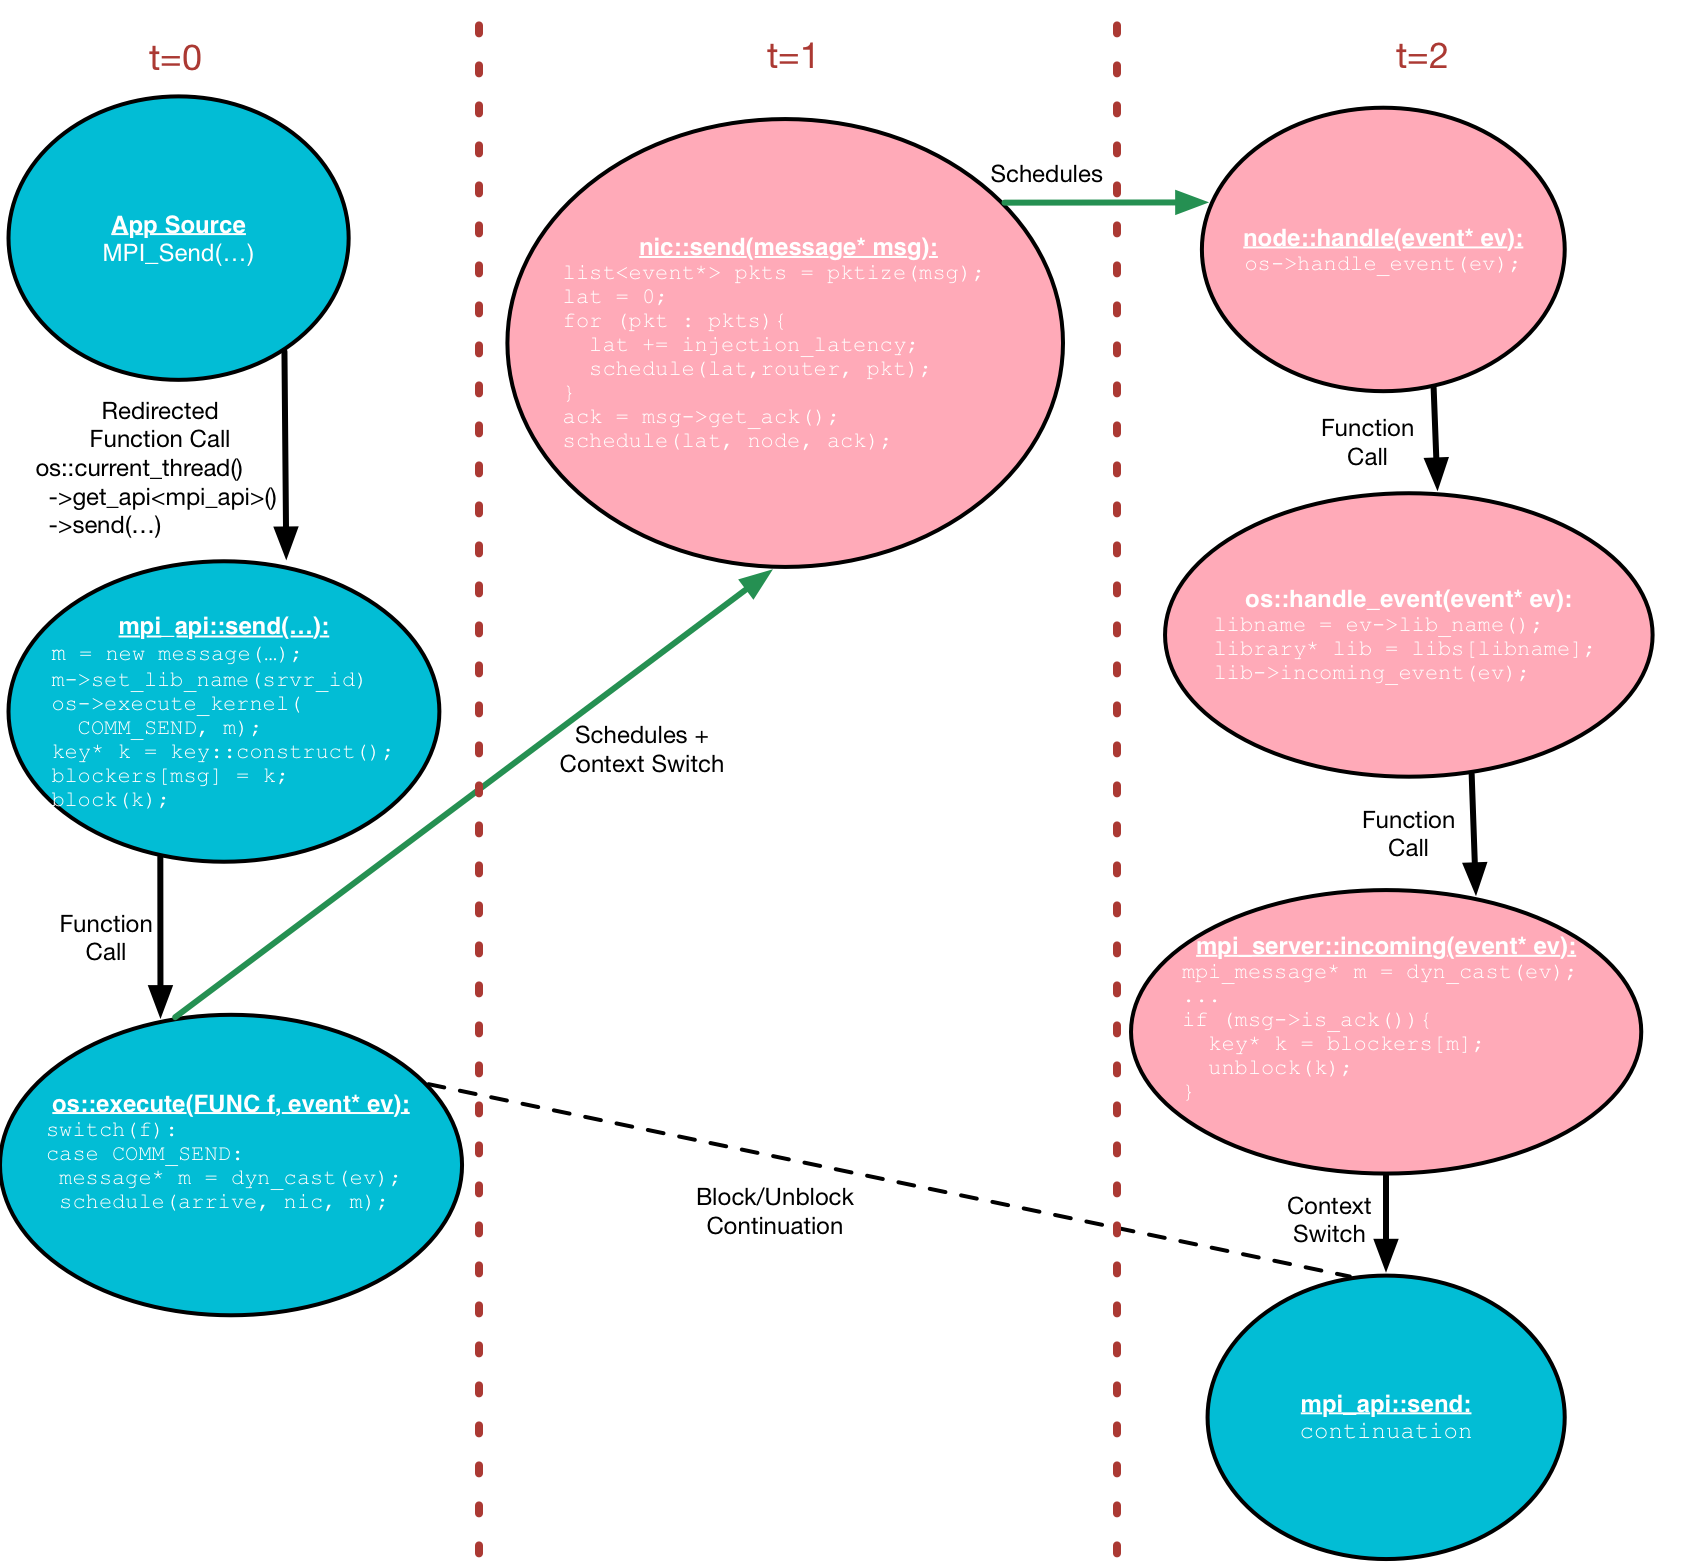
\includegraphics[width=1.05\textwidth]{figures/DES.png}
\caption{Flow of events for completing a send operation.  Shows basic function calls, block/unblock context switches, and event schedules. User-space thread (application) operations are shown in blue. Main event thread (OS/kernel) operations are shown in pink.}
\label{fig:desThreadsMPISend}
\end{figure}

When the ACK arrives back from the NIC, the ACK signals to MPI that the operation is complete allowing it to unblock.
The ACK is handled by a \inlinecode{service} object (which is the SST-specific implementation of an MPI server). 
A \inlinecode{service} is a special type of object, that we will discuss in more detail below.

\subsection{Thread-specific storage}
\label{subsec:threadStorage}
Let us look at the capture of the \inlinecode{MPI_Send} call. 
First, a macro redefines the call to avoid symbol clashes if using an MPI compiler (both virtual and real MPI cannot share symbols).
MPI uses global function calls to execute, meaning MPI has to operate on global variables.
However, SST/macro cannot use global variables.
Thus all state specific to each MPI rank (virtual thread) must be stashed somewhere unique.
This basically means converting all global variables into user-space thread-local variables.
When each user-space thread is spawned a \inlinecode{thread} object is allocated and associated with the thread.
This object acts as a container for holding all state specific to that virtual thread.
Rather than store MPI state in global variables, MPI state in stored in a class \inlinecode{MpiApi}, 
with one \inlinecode{MpiApi} object allocated per virtual MPI rank.
The operating system class provides a static function \inlinecode{currentThread} that makes the leap from
global variables to thread-local storage.
To access a specific API, a special helper template function \inlinecode{getApi} exists on each thread object.
Thus, instead of calling a global function \inlinecode{MPI_Send},
SST/macro redirects to a member function \inlinecode{send} on an \inlinecode{mpi_api} object that is specific to a virtual MPI rank.

\begin{table}
\def\arraystretch{1.5}
\begin{tabular}{>{\raggedright}p{2cm} >{\raggedright}p{3cm} >{\raggedright}p{3cm} >{\raggedright}p{3cm} >{\raggedright\arraybackslash}p{3cm}}
\hline
 & OS & Node & API & Service \\
\hline
Runs on Thread & 
  Both user-space and main DES thread &
  Only main DES thread (user-space with rare exceptions for optimization) &
%  Only main DES thread &
  Only user-space thread &
  Only main DES thread \\
How Advances Time & 
  Both blocking and scheduling events, depending on context &
  Scheduling events to other components &
%  Scheduling events to other components &
  Blocking or unblocking &
  Scheduling events to other components \\
Receives Events Via &
  Function calls from API/Service or from Node via \inlinecode{handle_event} function &
  Function calls from OS, receives scheduled events via the \inlinecode{handle} function &
%  Function calls from Node, receives scheduled events via \inlinecode{handle} function &
  Does not usually receive events - only blocks or unblocks &
  OS forwards messages to \inlinecode{incoming_event} function \\
Sends Events Via &
  Makes function calls and schedules events to Node &
  Makes function calls and schedules events to NIC, Memory &
%  Schedules events to Node, Interconnect &
  Does not usually send events - only blocks or unblocks &
  Makes function calls and schedules events to OS, unblocks APIs
\end{tabular}
\end{table}

\section{Libraries}
\label{sec:libraries}
The creating and handling of software events is managed through \inlinecode{library} objects.
Each \inlinecode{node} has an \inlinecode{OperatingSystem} member variable that will manage software events on a virtual compute node.
Each library object is stored in a lookup table in the operating system,
allowing the operating system to access specific libraries at specific times.

\begin{CppCode}
class OperatingSystem {
  ...
  map<string,Library*> libs_;
  ...
};
\end{CppCode}

Each library object has access to the operating system, being allowed to call

\begin{CppCode}
Event* ev = ...
os_->executeKernel(ty, ev);
\end{CppCode}
where an enum argument \inlinecode{ty} specifies the type of computation or communication and the event object carries all the data needed to model it.
This allows a library to \emph{call out} to the operating system.
Calls to \inlinecode{execute} \emph{always} occur on a user-space thread. 
In executing a computation or communication, the operating system may block inside \emph{execute} to advance time to complete the operation.
Calls to \inlinecode{execute_kernel} can occur on either a user-space thread or the main event thread.
Here the operating system acts as a service and \emph{never} blocks.

Conversely, each \inlinecode{library} must provide a \inlinecode{incomingEvent} method that allows the operating system to call back to the library

\begin{CppCode}
void incomingEvent(event* ev){...}
\end{CppCode}
Generally speaking, event notifications will arrive from the NIC (new messages, ACKs), memory system (data arrived), processor (computation complete), etc.
These hardware events must be routed to the correct software library for processing.

\begin{CppCode}
void OperatingSystem::handleEvent(event* ev) {
  library* lib = libs_[ev->libName()];
  lib->incomingEvent(ev);
}
\end{CppCode}
In order to route events to the correct library, the operating system maintains a string lookup table of \inlinecode{Library} objects.
All events associated with that library must be constructed with the correct string label, 
accessible through the event accessor function \inlinecode{libName}.

\subsection{API}
\label{subsec:softwareAPI}
The SST/macro definition of API was alluded to in \ref{subsec:threadStorage}.
The base \inlinecode{api} class inherits from \inlinecode{library}.
All API code must execute on a user-space thread.
API calls are always associated with a specific virtual MPI rank.
To advance time, API calls must block and unblock.
Functions executing on user-space threads are ``heavyweight'' in the sense that they consume resources.
API compute calls must allocate cores via a compute scheduler to execute.


API objects are accessible in skeleton apps through a global template function is provided in \inlineshell{sstmac/skeleton.h}.

\begin{CppCode}
template <class T>
T* getApi(const std::string& name);
\end{CppCode}
for which the implementation is

\begin{CppCode}
Thread* thr = OperatingSystem::currentThread();
return thr->getApi<T>(const std::string& name);
\end{CppCode}
which converts the global template function into a thread-specific accessor.
The most prominent example of an API is the \inlinecode{MpiApi} object for encapsulating an MPI rank.
Other prominent examples include the various computation APIs such as \inlinecode{BlasApi} that provides bindings for simulation various linear algebra functions.
